  \section{Artificial radial density bumps with a radially smooth
    viscosity profile}\label{add_sim}
  In \S\ref{density_bump} we found that vortices became stronger
  as the viscous layer thickness is increased, even though linear growth rates
  were reduced. Here, we present additional simulations to support the 
  hypothesis that this is due to the localised radial structure in the viscosity profile. 

  We repeated simulation V2 (see Table \ref{artificial_bump})
  with a radially-smooth viscosity profile given by 
  \begin{align}\label{smooth_visc}          
    \hat{\nu}\frac{\rho_i(R,z)}{B(R)} =
    \hat{\nu}_0\left[1+Q(z/H_0) \right]\frac{\rho_i(r_0,z)}{B(r_0)}. 
  \end{align}                  
  {\bf Recall the functions $B$ and $Q$ are given by Eq. \ref{bump_func} 
  and \ref{step}, respectively. 
  }
  We set the floor viscosity $\hat{\nu}_0=10^{-7}$ to mitigate
  axisymmetric viscous diffusion of the initial density bump. The
  viscous layer with $\hat{\nu} \sim 10^{-5}$ occupies $z\in[1,2]H_0$
  at $R=r_0$. {\bf This viscosity profile is shown in Fig. \ref{appen0}
  }  
                      
  \begin{figure}
  \centering
  \includegraphics[width=\linewidth]{figures/pdisk_visc2d_appendix.ps}
  \caption{{\bf The radially-smooth viscosity profile given by Eq. \ref{smooth_visc}.
         This plot is to be compared with Fig. \ref{visc2d}.\label{appen0}}}
  \end{figure}


  This simulation is shown as the dotted line in Fig. \ref{appen} in
  terms of the $m=1$ component of the kinetic energy density. We
  compare it to the corresponding case using the radially-structured
  viscosity profile in \S\ref{density_bump} {\bf (i.e. the original case V2 but with
  lowered floor viscosity)}. Vortex formation occurs
  in both runs.  
  With a radially-smooth viscosity profile, the vortex decays 
  monotonically after $|W_1|$ reaches maximum value of $\sim 0.05$. 
  Using the radially-structured viscosity profile (solid line) gives a
  larger disturbance amplitude at the linear stage  ($\max{|W_1|}\sim
  0.08$), and although it subsequently decays, the decay is halted for
  $t\gtrsim110P_0$.    

  The contrast between these cases show that the radial structure
  in the viscosity profile helps vortex survival. This experiment
  indicates that the dominant effect of viscosity is its
  influence on the evolution of the axisymmetric part of background
  disc. The radially-structured viscosity profile is a source for the
  radial PV minimum, which is needed for the RWI.  

  Our result here is qualitatively similar that in \cite{regaly12},
  where a sharp viscosity profile was imposed in a 2D simulation and 
  vortex formation ensues via the RWI. The vortex eventually
  disappears, but re-develops after the system returns to {\bf an}
  axisymmetric state. This is because the imposed viscosity profile
  causes the disc to develop the required PV minimum for the RWI. 

 \begin{figure}
  \centering
  %  \includegraphics[scale=.41,clip=true,trim=0cm 1.cm 0cm 0cm]{figures/pdisk_kerz_cases_appendix.ps}
  \includegraphics[width=\linewidth]{figures/pdisk_kerz_cases_appendix1.ps}
  \caption{Evolution of the $m=1$ component of the kinetic energy
    density, averaged over the shell $r\in[0.8,1.2]r_0$, for a layered 
    disc initialised with a radial density bump. 
    The solid line employs the {\bf radially-structured} viscosity profile given by 
    Eq. \ref{visc_profile} {\bf (see Fig.\ref{visc2d}). The} dotted line employs the radially-smooth
    viscosity profile given by Eq. \ref{smooth_visc} {\bf and shown in Fig. \ref{appen0}}. \label{appen} }
  \end{figure}
